\documentclass[a4paper,11pt]{exam}
%\printanswers % pour imprimer les réponses (corrigé)
\noprintanswers % Pour ne pas imprimer les réponses (énoncé)
\addpoints % Pour compter les points
% \noaddpoints % pour ne pas compter les points
%\qformat{\textbf{\thequestion ) } }
\qformat{\textbf{\thequestion )} (\thepoints) \\} % Pour définir le style des questions (facultatif)
\usepackage{color} % définit une nouvelle couleur
\shadedsolutions % définit le style des réponses
% \framedsolutions % définit le style des réponses
\definecolor{SolutionColor}{rgb}{0.8,0.9,1} % bleu ciel
\renewcommand{\solutiontitle}{\noindent\textbf{Solution:}\par\noindent} % Définit le titre des solutions




\makeatletter

\def\maketitle{{\centering%
	\par{\huge\textbf{\@title}}%
	\par{\@date}%
	\par}}

\makeatother

\lhead{NOM Pr\'enom :}
\rhead{\textbf{Les r\'eponses doivent \^etre justifi\'ees}}
\cfoot{\thepage / \pageref{LastPage}}


%\usepackage{../../pas-math}
%\usepackage{../../moncours}


%\usepackage{pas-cours}
%-------------------------------------------------------------------------------
%          -Packages nécessaires pour écrire en Français et en UTF8-
%-------------------------------------------------------------------------------
\usepackage[utf8]{inputenc}
\usepackage[frenchb]{babel}
\usepackage[T1]{fontenc}
\usepackage{lmodern}
\usepackage{textcomp}



%-------------------------------------------------------------------------------

%-------------------------------------------------------------------------------
%                          -Outils de mise en forme-
%-------------------------------------------------------------------------------
\usepackage{hyperref}
\hypersetup{pdfstartview=XYZ}
%\usepackage{enumerate}
\usepackage{graphicx}
\usepackage{multicol}
\usepackage{tabularx}
\usepackage{multirow}


\usepackage{anysize} %%pour pouvoir mettre les marges qu'on veut
%\marginsize{2.5cm}{2.5cm}{2.5cm}{2.5cm}

\usepackage{indentfirst} %%pour que les premier paragraphes soient aussi indentés
\usepackage{verbatim}
\usepackage{enumitem}
\usepackage[usenames,dvipsnames,svgnames,table]{xcolor}

\usepackage{variations}

%-------------------------------------------------------------------------------


%-------------------------------------------------------------------------------
%                  -Nécessaires pour écrire des mathématiques-
%-------------------------------------------------------------------------------
\usepackage{amsfonts}
\usepackage{amssymb}
\usepackage{amsmath}
\usepackage{amsthm}
\usepackage{tikz}
\usepackage{xlop}
%-------------------------------------------------------------------------------



%-------------------------------------------------------------------------------


%-------------------------------------------------------------------------------
%                    - Mise en forme avancée
%-------------------------------------------------------------------------------

\usepackage{ifthen}
\usepackage{ifmtarg}


\newcommand{\ifTrue}[2]{\ifthenelse{\equal{#1}{true}}{#2}{$\qquad \qquad$}}

%-------------------------------------------------------------------------------

%-------------------------------------------------------------------------------
%                     -Mise en forme d'exercices-
%-------------------------------------------------------------------------------
%\newtheoremstyle{exostyle}
%{\topsep}% espace avant
%{\topsep}% espace apres
%{}% Police utilisee par le style de thm
%{}% Indentation (vide = aucune, \parindent = indentation paragraphe)
%{\bfseries}% Police du titre de thm
%{.}% Signe de ponctuation apres le titre du thm
%{ }% Espace apres le titre du thm (\newline = linebreak)
%{\thmname{#1}\thmnumber{ #2}\thmnote{. \normalfont{\textit{#3}}}}% composants du titre du thm : \thmname = nom du thm, \thmnumber = numéro du thm, \thmnote = sous-titre du thm

%\theoremstyle{exostyle}
%\newtheorem{exercice}{Exercice}
%
%\newenvironment{questions}{
%\begin{enumerate}[\hspace{12pt}\bfseries\itshape a.]}{\end{enumerate}
%} %mettre un 1 à la place du a si on veut des numéros au lieu de lettres pour les questions 
%-------------------------------------------------------------------------------

%-------------------------------------------------------------------------------
%                    - Mise en forme de tableaux -
%-------------------------------------------------------------------------------

\renewcommand{\arraystretch}{1.7}

\setlength{\tabcolsep}{1.2cm}

%-------------------------------------------------------------------------------



%-------------------------------------------------------------------------------
%                    - Racourcis d'écriture -
%-------------------------------------------------------------------------------

% Angles orientés (couples de vecteurs)
\newcommand{\aopp}[2]{(\vec{#1}, \vec{#2})} %Les deuc vecteurs sont positifs
\newcommand{\aopn}[2]{(\vec{#1}, -\vec{#2})} %Le second vecteur est négatif
\newcommand{\aonp}[2]{(-\vec{#1}, \vec{#2})} %Le premier vecteur est négatif
\newcommand{\aonn}[2]{(-\vec{#1}, -\vec{#2})} %Les deux vecteurs sont négatifs

%Ensembles mathématiques
\newcommand{\naturels}{\mathbb{N}} %Nombres naturels
\newcommand{\relatifs}{\mathbb{Z}} %Nombres relatifs
\newcommand{\rationnels}{\mathbb{Q}} %Nombres rationnels
\newcommand{\reels}{\mathbb{R}} %Nombres réels
\newcommand{\complexes}{\mathbb{C}} %Nombres complexes


%Intégration des parenthèses aux cosinus
\newcommand{\cosP}[1]{\cos\left(#1\right)}
\newcommand{\sinP}[1]{\sin\left(#1\right)}


%Probas stats
\newcommand{\stat}{statistique}
\newcommand{\stats}{statistiques}
%-------------------------------------------------------------------------------

%-------------------------------------------------------------------------------
%                    - Mise en page -
%-------------------------------------------------------------------------------

\newcommand{\twoCol}[1]{\begin{multicols}{2}#1\end{multicols}}


\setenumerate[1]{font=\bfseries,label=\textit{\alph*})}
\setenumerate[2]{font=\bfseries,label=\arabic*)}


%-------------------------------------------------------------------------------
%                    - Elements cours -
%-------------------------------------------------------------------------------





%\usepackage{fullpage}
\author{\ }
\date{25 Septembre 2019}
\title{$5^e G$ : DS num\'ero 1}


\begin{document}
%	\usepackage{fancyhdr}
%	
%	\pagestyle{fancy}
%	\fancyhf{}
	%\rhead{Share\LaTeX}

	\maketitle
	
\begin{center}
	\textbf{Calculatrice interdite}
\end{center}

\begin{small}
	\begin{center}
		\begin{tabular}{|@{\ }l@{\ }|@{\ }c@{\ }|@{\ }c@{\ }|@{\ }c@{\ }|@{\ }c@{\ }|}
			\hline
			\textbf{Compétence} & \textbf{MI} & \textbf{MF} & \textbf{MS} & \textbf{TBM} \\
			\hline
			\textbf{Calculer} (Calculer une expression numérique) (Ex 2, question 1)&  \ \ & \ \ & \ \ & \ \  \\
			\hline	
			\textbf{Modéliser} (Traduire une situation réelle en langage mathématique) (Ex 4)& \ \ & \ \ &  \ \  & \ \ \\
			\hline
%			 \textbf{Communiquer} (Expliquer sa démarche, son raisonnement ) &  \ \ & \ \ & \ \ & \ \  \\
%			\hline
		\end{tabular}
	\end{center}
\end{small}	

	
	
\section{Arbres de calcul (6 points)}

\begin{questions}
	\question[3] Décrire par une phrase les arbres de calcul suivant et écrire l'expression correspondante (le résultat n'est pas demandé).
	
	
	\begin{center}
		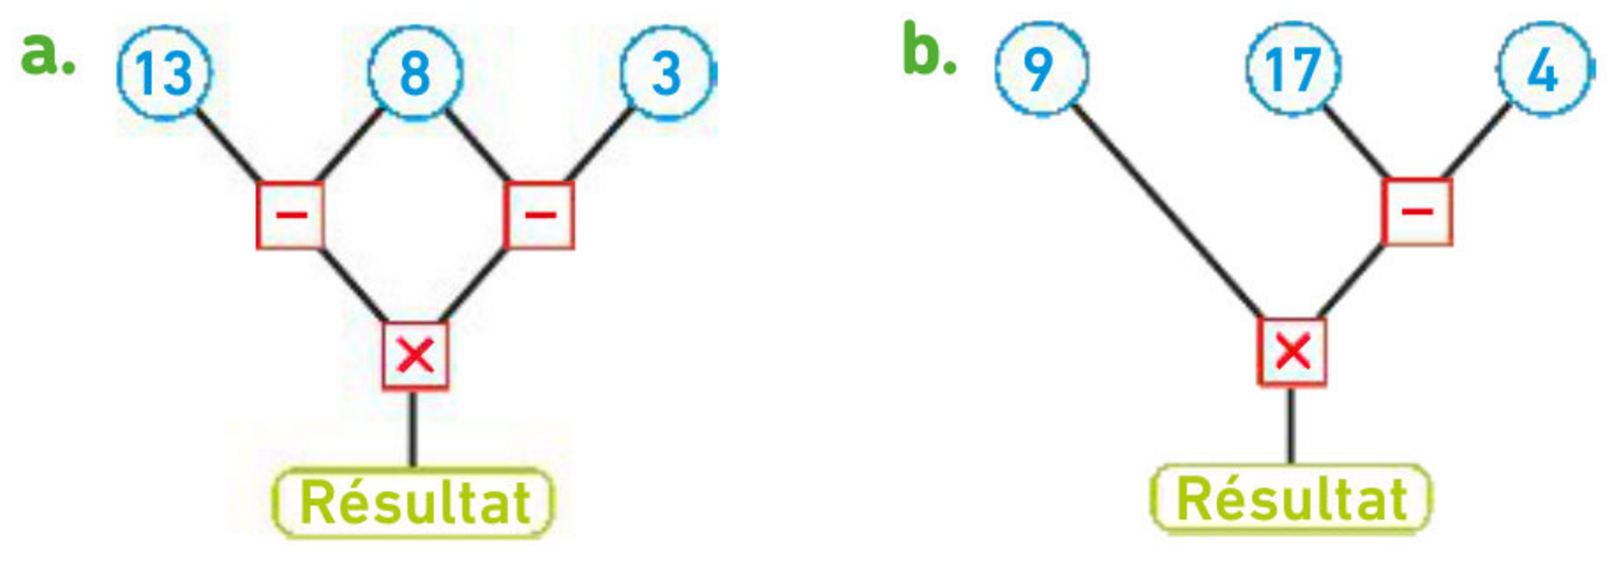
\includegraphics[scale=0.3]{img/arbres}
	\end{center}
	
	\begin{solution}
		\begin{enumerate}
			\item Cet arbre correspond au produit de la différence de 13 et 8 et de celle de 8 et 3. ($(13 - 8) \times (8 - 3)$).
			
			\item Cet arbre correspond au produit de 9 par la différence de 17 et 4. ($9 \times (17 - 4)$).
		\end{enumerate}
	\end{solution}
	\question[3] Décrire par une phrase les expressions suivantes et dessiner l'arbre de calcul correspondant.
	
	\begin{multicols}{2}
		\begin{enumerate}
			\item $30 \times 4 + 20 \div 2$
			\item $30 \times (20 - 4)$
			%\item $10 + 4 \times 10$
		\end{enumerate}
	\end{multicols}	

	
	\begin{solution}
		\begin{multicols}{2}
			\begin{enumerate}
				\item Cette expression correspond à la somme du produit de 30 et 4 et du quotient de 20 par 2.
					
				\item Cette expression correspond au produit de 30 par la différence de 20 et 4.
			\end{enumerate}
		
		\end{multicols}
	\end{solution}
	
\end{questions}
	

\section{Calculer (8 points)}


\begin{questions}
	\question[4] Calculer les expressions suivantes en détaillant tous les calculs :
	
	\begin{enumerate}
		\item $A = 62 - 30 - 7 + 20$
		
		\item $B = (50 - (13 + 1) \times 2) - 6$
		
		\item $C= 225 - ((15 + 7) \times 10 - 2)$
		
		\item $D= (10 \times \num{3.2} - (79 - 71)) \div 6$
	\end{enumerate}


	\begin{solution}
		
		\begin{multicols}{2}
			
		\begin{eqnarray*}
			A &=& 62 - 30 - 7 + 20 \\
			A &=& 32 - 7 + 20 \\
			A &=& 25 + 20 \\
			A &=& 45
		\end{eqnarray*}
		
		\begin{eqnarray*}
			B &=& (50 - (13 + 1) \times 2) - 6 \\
			B &=& (50 - 14 \times 2) - 6  \\
			B &=& (50 - 28) - 6  \\
			B &=& 22 - 6  \\
			B &=& 37
		\end{eqnarray*}
		
		\begin{eqnarray*}
			C &=& 225 - ((15 + 7) \times 10 - 2)\\
			C &=& 225 - (22 \times 10 - 2) \\
			C &=& 225 - (220 - 2) \\
			C &=& 225 - 218  \\
			C &=& 7
		\end{eqnarray*}
		
		\begin{eqnarray*}
			D &=& (10 \times \num{3.2} - (79 - 71)) \div 6\\
			D &=& (10 \times \num{3.2} - 8) \div 6 \\
			D &=& (32 - 8) \div 6 \\
			D &=& 24 \div 6  \\
			D &=& 4
		\end{eqnarray*}
		\end{multicols}
	\end{solution}

	\question[1] Placer des parenthèses dans $A = 62 - 30 - 7 + 20$ pour trouver 59.
	\begin{solution}
		\begin{eqnarray*}
			A &=& 62 - (30 - 7) + 20 \\
			A &=& 62 - 23 + 20 \\
			A &=& 39 + 20 \\
			A &=& 59
		\end{eqnarray*}
	\end{solution}
	
	\question[1] Placer des parenthèses dans $A = 62 - 30 - 7 + 20$ pour trouver 19.
	\begin{solution}
		\begin{eqnarray*}
			A &=& 62 - (30 - 7 + 20) \\
			A &=& 62 - (23 + 20) \\
			A &=& 62 - 43\\
			A &=& 19
		\end{eqnarray*}
	\end{solution}
\end{questions}

%\section{Station spatiale (3 points)}

La station spatiale Mir est restée sur orbite pendant 15 ans et a fait à peu près \num{86500} fois le tour de la Terre pendant la durée de son vol spatial.

Le record du plus long séjour dans l'espace revient à Valéri Poliakov qui a vécu 438 jours d'affilée sur Mir.

\begin{questions}
	\question[1\half] Comment faire pour calculer le nombre de fois que ce cosmonaute a fait le tour de la Terre ? (On demande d'expliquer la méthode, pas de faire le calcul.)
	
	
	\question[1\half] \'Ecrire les calculs à faire en une seule expression ? (le résultat n'est pas attendu)
\end{questions}

\section{Expressions (5 points)}

Pour chacune des deux situations suivantes, écrire une seule expression permettant de répondre à la question posée :

\begin{questions}
	\question[1\half] Emma a acheté trois livres identiques et a payé 36 €. Vincent qui avait 150 €, achète un de ces livres. Quelle somme reste-t-il à Vincent ?
	
	\question[1\half] Dans une planche de 150 cm de long, Paul découpe trois morceaux de 36 cm de long. Quelle longueur reste-t-il ?
	
	\question[2] Théo doit lire un livre de 150 pages. Le lundi il lit 36 pages. Il le termine en lisant le même nombre de pages chacun des trois jours suivants. Combien de pages a-t-il lu chacun de ces trois jours ?
\end{questions}

\section{Sucreries (3 points bonus)}

Magali achète 7 paquets de gâteaux à \num{1.50} € pièce et 14 sucettes à \num{0.50} € pièce. Elle a payé avec un billet de 20 €.

\begin{questions}
	\question[\half] Que représente le calcul $14 \times \num{0.50}$ ?

	\question[\half] Que représente le calcul $7 \times \num{1.50}$ ?
	
	\question[1] En n'utilisant que les nombres écrits dans l'énoncé écrire l'expression permettant de calculer la monnaie que la caissière lui rendra. (le résultat n'est pas attendu)
		
	\question[1] Effectuer le calcul et conclure. 

	
\end{questions}

\label{LastPage}

%\section{Consommation électrique}
%
%Une consommation d'électricité se mesure en 
\end{document}